\lhead{\emph{Conclusion}}
\chapter{Conclusion}\label{ch:conclusion}



\section{Key Findings}

%\begin{itemize}
%\item I was given a kind-of working prototype and a copy of Bea's thesis, and I was told to ``make it work''.  It works, now.  Really, really well.  So, the project was a complete success.
%\item Along the way, I discovered a whole bunch of new problems.  I solved each problem and improved the system considerably each time.
%\item We need to list here the main important improvements and results.  It should mimic the list at the start of Chapter 5, probably.
%\end{itemize}

My MSc thesis work was initiated with the goal of establishing a
working multi-dimensional PID control system for magnetic fields,
based on the work of Refs.~\cite{bea} and~\cite{lins}.  This goal was
successfully achieved and the work went beyond the goal in several
respects.  In the process of developing the system, I discovered a host
of new challenges, to which I found innovative solutions.  Below I
least the key improvements made to the system and the results of those
improvements.  They are:
\begin{enumerate}
\item {\bf $\mathbf{4^{th}}$ order low pass Butterworth filter.}  I designed 12 active filters which are excellent in reducing high frequency noise even slightly better than the low pass filter (LPF) of Bartington's SCU. The filters will be important for any types of future studies with high frequency noise issue. The filters can be improved by designing them in multi-gain pattern instead of constant gain that I have built. The advantage of multi-gain is that if the signal is very small (smaller than the lowest that an ADC can read) then the signal can be read by multiplying it with a larger gain. In my case, to acquire the fluxgate signals placed inside the shield within the coil cube, I have used LPF of Bartington's SCU with gain of 100 which boost the signal 100 times so that can be easily read by the ADC.  

\item {\bf Prototype PI control simulation.}  The simulation of the prototype active compensation system is vital to demonstrate a full understanding of the experimental results. The static part of the simulation involves FEA simulation in OPERA to produce field maps within the coil cube to generate the matrix $\bm{M}$ and the field change $\Delta B$ due to perturbation coil for any number of the sensors placed within the coil cube. This will be a very handy tool for the future students as they will have the freedom to use thousands of sensors within their respective cube dimension and most importantly they do not have to worry about placing the sensors correctly in their system to study in detail about the effect of $\bm{M}$ for any set of sensors. The dynamic part of the simulation involves time dependent PI feedback algorithm in Python. Implementing the values of static part in dynamic part generates a real time PI control simulation which gives very good results compared to experiment (see Fig.~\ref{fig:exp_sim}).  Simulation of a certain system integrating feedback algorithm is a unique work that has not been still published in any thesis related to active compensation. I could have avoided many problems observed in the data, {\it e.g.} the current drifting problem, before ever using the system if this simulation had existed a priori. Even the simulation in free space (not requiring OPERA) would have shown many of the same issues. The strong message for future work is to use this kind of simulation as a tool for testing the entire system before it is built.


%\begin{itemize}
%\item OPERA part (static)
%\item PI part (dynamic)
%\item Putting them together gives very good results compared to experiment.
%\item Main proposal for future work is to use this kind of simulation as a tool for testing the entire system before it is built.
%\item Many problems observed in the data, e.g. the current drifting problem, could have been found before ever using the system if this simulation had existed a priori.
%\item Even simulation in free space (not requiring OPERA) would have shown many of the same issues.
%\end{itemize}

\item {\bf Better understanding of matrix inversion, PI parameters, and tuning.} The author in Ref.\cite{bea} proposed a matrix inversion with Tikhonov regularization which I have blindly followed initially. But I have realized later that there is more to the story than just having matrix inversion and PI tuning {\it i.e.} there is a relationship between the regularization parameter $r$ and PI parameters and studied this in more details. I came to the conclusion that no amount of PI tuning can reduce the current drifting problem even though $r$ is optimized properly.  However, the current drifting problem can be reduced by adjusting $r$ and PI parameters treating $r$ more-or-less another free parameter. But this introduces high frequency noise which gave me the clear understanding to describe Eqs.~(\ref{eq:del_I_pseudo}), and ~(\ref{eq:tikhonov}). Moreover, I have also proposed a new method to find $r$ based on the condition number of the matrix which I think more robust than the method described by the author in Ref.\cite{bea}. Eventually, I have realized that implementing regularized matrix inversion is a waste of time. I will strongly suggest to avoid an ill-conditioned matrix which I should say that I have been somewhat advised by Ref.~\cite{rawlikpriv} in a conversation while attending nEDM workshop in 2017. 

Although I have got some good advice from Ref.~\cite{rawlikpriv}, but I was not sure about the author's proposal of a new feedback algorithm not based on PI which the author claimed in Ref.~\cite{rawlik}. I showed that this is equivalent to a PI system restricted to one particular choice of tuning.  It is clearly better to allow more flexibility in the tuning than feedback algorithm proposed by the author in Ref.~\cite{rawlik}.


%\begin{itemize}
%\item Bea did matrix inversion.  I realized there's a relationship between the matrix regularization and PI parameters and studied this in more details.
%\item Rawlik proposed a new feedback algorithm apparently not based on PI.  I showed that this is equivalent to a PI system restricted to one particular choice of tuning.  It is clearly better to allow for more flexibility in the tuning than proposed by Rawlik.
%\end{itemize}

\item {\bf Coil current modes based on coil configuration.}  Solving the current drifting problem was the breakthrough of this thesis. Because while searching for the solution, I have built very efficient filters and realized that passive shield has no impact on final active compensation result, and regularization is a waste of time, made an useful tool {\it i.e.} simulation to test the system and finally able to solve by understanding the coil current pattern for different coil configuration. The simulation in free space found to be very effective understanding the problem. I have discovered that while using 6~coil feedback algorithm there is one mode which cancels current coming out of other coils essentially makes the system ineffective producing closer to zero singular value $\sigma_n$ of $\bm{M}$. That is why the system is always ill-conditioned {\it i.e.} large condition number of $\bm{M}$. I then  wired up two coils to make the prototype run on 5~coil feedback algorithm which cancels the bad coil current mode producing close to one condition number of $\bm{M}$ forcing the system well-conditioned. It was then I realized I did not need to regularize the system if the system is well conditioned in the first place. So, I strongly agree with the author in Ref.~\cite{rawlik} on low condition number as a measure of good system performance. As coil designing is beyond the scope of this thesis, I will suggest future researchers interested to work on active compensation is that make the system well conditioned by studying different coil design or discover new coil design before anyone want to use the feedback algorithm.
%\begin{itemize}
%\item Agreement with Rawlik on low condition number as a measure of good system performance.  This will be another recommendation for future work on coil design:  to make sure the condition number is reasonable.
%\end{itemize}
\end{enumerate}



\section{Recommendations on Design for TUCAN nEDM Experiment}

\begin{enumerate}
\item Take the attitude that you are supervising the next person to work on this.  What is the first thing they should do?  The next thing?  How to bring the design process to a conclusion so that the system could be built.
\item discussion on better ideas beyond regularization, such as spherical harmonics, patch coils, and how this can lead to a properly regularized system that is more flexible
\item Designing the system for the known perturbations... at TRIUMF, what are they?  This can be used as an input to the design process.  Relate back to the $C_x^\pm$ data.
\item Small condition number is not the most important thing.  We can get small condition number if only three coils are used.  But this system will only be able to cancel uniform fields.
\item Use spherical harmonics to the desired order and use coils or restricted combinations of coils to mimic those spherical harmonics.  The restricted set of coil currents should then be well-conditioned.  Rawlik went beyond this and suggested rewiring patch coils to generate spherical harmonics more efficiently.
\item Discussion on simulation and simulating the system ``fully'' (including the PI loop) using the tools you developed before beginning to build it.  Should make the point that we now know enough to do a good job a priori.
\end{enumerate}


% I strongly recommend that do not waste time regularized an ill-conditioned system (large condition number) rather spend time on building a well-conditioned system (small condition number). The author in Ref.~\cite{rawlik} is also vocal on small condition number. 
As discussed in Chapter~\ref{ch:magnetics}, the TUCAN nEDM experiment is located next to TRIUMF cyclotron with $\sim400~\mu$T background, $\sim100$~nT fluctuations, and $100~\mu$T/m gradients. Moreover, the 50 ton crane in the experimental site can also induces very large changes. The perturbations must be quantified properly. I recommend to build a well-conditioned system where the perturbation can be used as an input to the design process. I discourage to justify the design process by considering having small condition number only. Because, small condition number can easily be generated if only three coils are used but then the system having three coils will be restricted to cancel only uniform fields ignoring gradients. Hence, I rather suggest to use spherical harmonics to the desired order and use coils or restricted combinations of coils to mimic those spherical harmonics. The restricted set of coil currents should then be well-conditioned. I have already showed the restricted set of coil currents in Section~\ref{sec:coil_config} which decreases the condition number for my system significantly. The author in Ref.~\cite{rawlik} went beyond this and suggested rewiring patch coils to generate spherical harmonics more efficiently and described a coil design method in Ref.~\cite{rawlik_paper_coil}. A well conditioned system is more flexible as it does not have to worry about regularization and it exactly knows the value coil currents to eliminate a certain field in certain direction.

% \textcolor{red}{Designing the system for the known perturbations... at TRIUMF, what are they?  This can be used as an input to the design process.  Relate back to the $C_x^\pm$ data.  }

Having the system defined properly by improved coil design based on spherical harmonics and known perturbation, I recommend to make the simulation of the system integrating the PI feedback algorithm using the tools that I developed before beginning to build it. The simulation will give the full picture of what is expected and what the system is offering and if that are not aligned make sure to correct the design and confirm again via simulation before building the system. Making a simulation beforehand should make the point that thes system has been understood and tested enough to do a good job a priori.
% Discussion on simulation and simulating the system ``fully'' (including the PI loop) using the tools you developed before beginning to build it.  Should make the point that we now know enough to do a good job a priori.







\section{Implementation in the TUCAN nEDM Experiment}

\begin{itemize}
\item Requirements... we need 'em.  Cite PSI conference proceeding which says we ``might'' implement such a system in n2EDM.  Trade-offs of active vs.~passive shielding and the decision on the dividing line between the two.  History of the PSI system.
\item Engineering statements...  we have to be able to build it and make it fit
\item Other applications of active shield:
\begin{itemize}
\item Saturation?
\item Providing a somewhat smaller field when the door to the room is opened?
\item Somewhat smaller field to prepare components for the room?
\end{itemize}
\end{itemize}



The first and foremost question is to be answered is that whether we need active compensation system or not. PSI group has already commissioned an active compensation system~\cite{bea_paper} for their previous nEDM experiment in 2013 because of having the experiment closer to facilities generating strong magnetic fields which induce $\Delta B$ at the experiment location of up to tens of $\mu$T on time scales from minutes to hours. Their present experiment namely ``n2EDM'' is also located around the same place and the n2EDM experimental volume is shielded from these perturbations by the MSR, but they ``might be left with measurable changes in the magnetic field of the experiment'' as quoted in Ref.~\cite{psi_n2edm_PPNS-workshop}. They are developing an active compensation system as an additional shielding layer and ''might be installed after initial characterization measurements'' quoted in same Ref.~\cite{psi_n2edm_PPNS-workshop}. 

\fig{Images/active_scheme}{width = 0.8\textwidth}{Schematic diagram for the TUCAN nEDM magnetics. From inside out: The UCN and the co-magnetometers followed by the internal coil system ($\bm{B_0}$ and $\bm{B_1}$ coils) to generate the magnetic fields for the Ramsey cycle. Outside to that there are four layers of passive shielding which made the magnetically shielded room (MSR). The active compensation system which needs to be designed is just outside the MSR.\label{fig:msr_zoomed}}{Schematic diagram for the TUCAN nEDM magnetics 2}

%  At large fields, saturation of the passive magnetic shielding system can be a concern, which would seriously impact its effectiveness. Furthermore, when accessing the experiment, the door to the MSR must be opened. If presented with a large external field, the innermost layer of the passive shielding system could themselves become magnetized, necessitating degaussing and additional experimental down time with these factors in mind. The proposed plan is to nullify and stabilize the magnetic field environment at TRIUMF to ($\sim\;1\;\mu T$) using dedicated large bucking coils and also to reduce the fluctuations upto a factor of 100 using a separate set of coils by supplying currents to them  where the fluctuations will be measured by fluxgate sensors in a continuous feedback loop.



As to decide the need of active compensation for TUCAN nEDM experiment, it is first required to analyze the following statements :
\begin{enumerate}
    \item {\bf Trade-offs of active vs.~passive shielding and the decision on the dividing line between the two.} Both the active and passive shielding are expensive, but it’s not clear as of yet what costs more, an additional layer of mu-metal or a compensation coil system. Advantage of coils: allows to compensate DC magnetic fields which improves the performance of MSR and long term stability of $\bm{B_0}$ field inside the MSR; disadvantage: complex system which requires a lot of development and constant monitoring and analysis until proven to operate stably as good as possible. It is noteworthy to mention that active shields do not replace passive ones. For very low frequencies {\it i.e. $\mathrm{<~Hz}$}, the shielding factor of passive shields degrades~\cite{active_raw_app_0,active_raw_app_1}. Meanwhile, the performance of active shields are best best at DC and reach up to $\mathrm{KHz}$. A stable magnetic field over the whole range of frequencies is expected from the combination of the two shielding methods~\cite{active_raw_app_0,active_raw_app_1,active_raw_app_2,active_raw_app_3}.
    
    \item {\bf Saturation.} At large fields, saturation of the passive magnetic shielding system comprising the MSR as shown in Fig.~\ref{fig:msr_zoomed} can be a concern, which would seriously impact its effectiveness. The companies that offer MSR will not give a written specification that the equipment delivered by them will perform the same when in a field significantly larger than earth fields. The performance of MSR must be tested first and we should be satisfied fully that the MSR's performance will not be hampered in the field conditions more larger than the MSR has been specified for.
    
    % So looking at it from a legal point of view, it would probably be a good idea for the case we ever wanted to complain about the performance of the MSR that we can show that we operate it in the conditions it has been specified for.

    \item {\bf Providing a somewhat smaller field when the door to the room is opened.} When accessing the experiment, the door to the MSR must be opened. If presented with a large external field, the innermost layer of the passive shielding system could themselves become magnetized, necessitating degaussing and additional experimental down time with these factors in mind.
    \item {\bf Somewhat smaller field to prepare components for the room?}
    \item {\bf Engineering statements.} From engineering point of view, it should clearly states about the possibility of building it and making it in the experimental site.
\end{enumerate}


The discussion on above statements will help us decide about whether we need an active compensation system or not.

 

% \subsubsection{Effect of changing only P term}
% Here, the effect of changing proportional gain term (P) or $k_c^p$ of Eq.~(\ref{eq:I}) will be discussed.

% P term is proportionally multiplying the error (the difference between setpoint and actual measurement) with a constant gain. For the prototype it is

% \begin{equation}
%     P_{\text{PI}}=k_c^p \Delta I_c^n
% \end{equation}
% where, $k_c^p$ is the proportional gain and $\Delta I_c^n$ is explained in Eq.~(\ref{eq:del_I}).

% Depending on the value $k_c^p$, it tries to minimize the error level between the setpoint and the actual measurement with passage of several measurements. A large value of $k_c^p$ will result large output change for a particular error and eventually it reaches a threshold point above which the system becomes unstable. 

% % \begin{figure}[!htb]
% %     \begin{subfigure}{.5\linewidth}
% %         \centering
% %         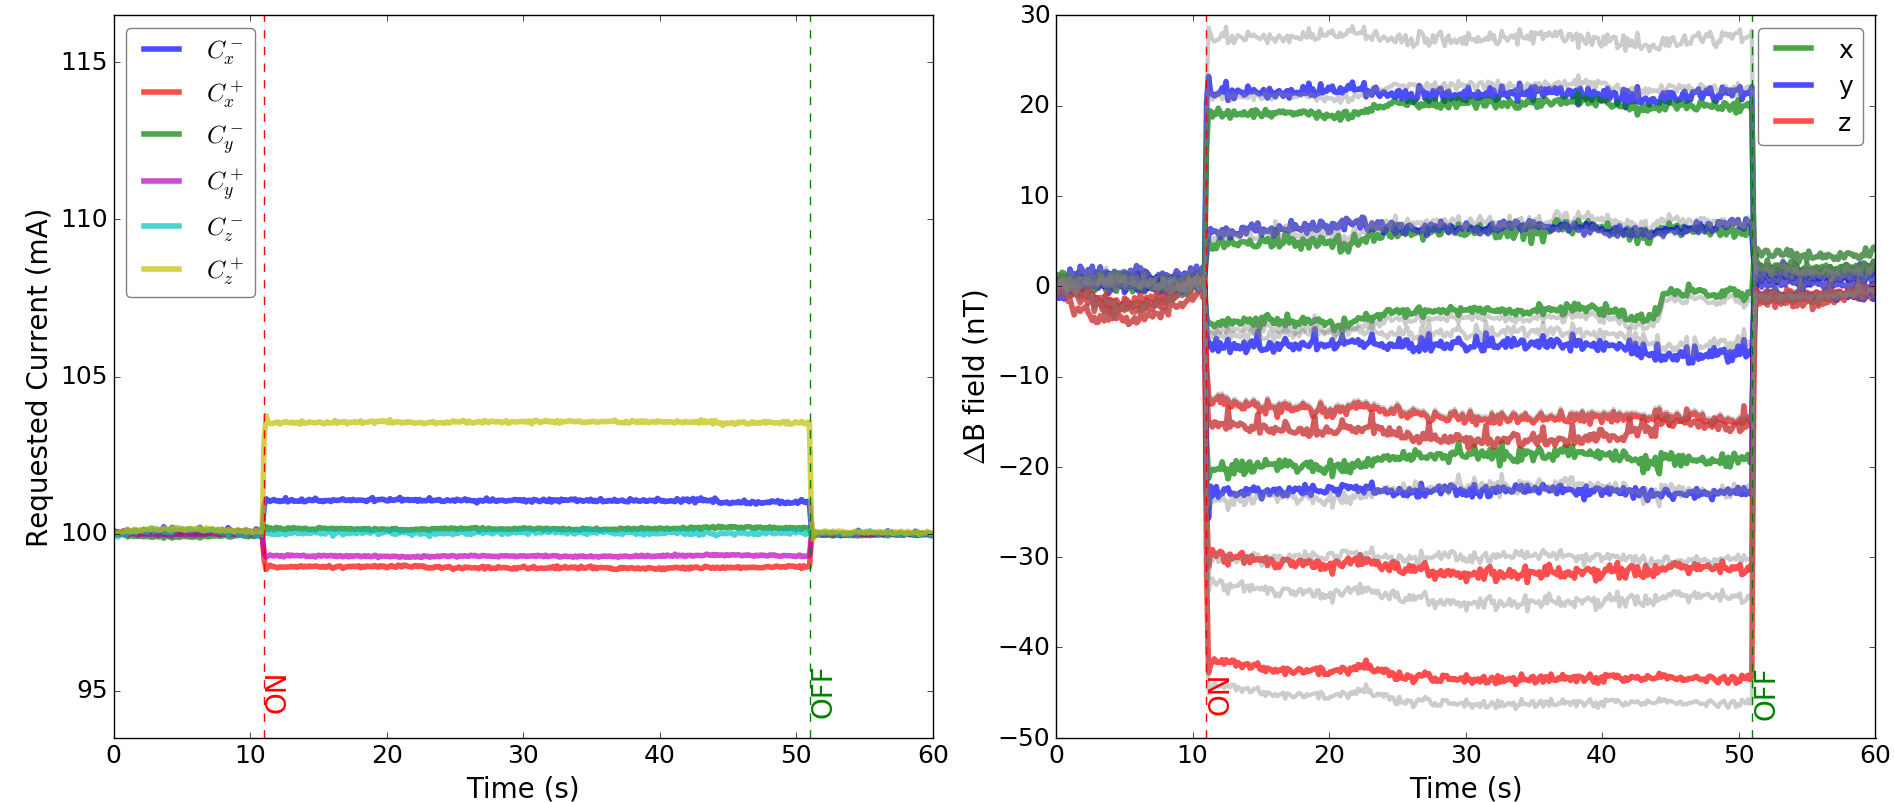
\includegraphics[width=\linewidth, height= 6.5 cm]{Images/p25}
% %         \caption{at $k_c^p$=0.25}
% %         \label{fig:p25}
% %     \end{subfigure}%
% %     \begin{subfigure}{.5\linewidth}
% %         \centering
% %         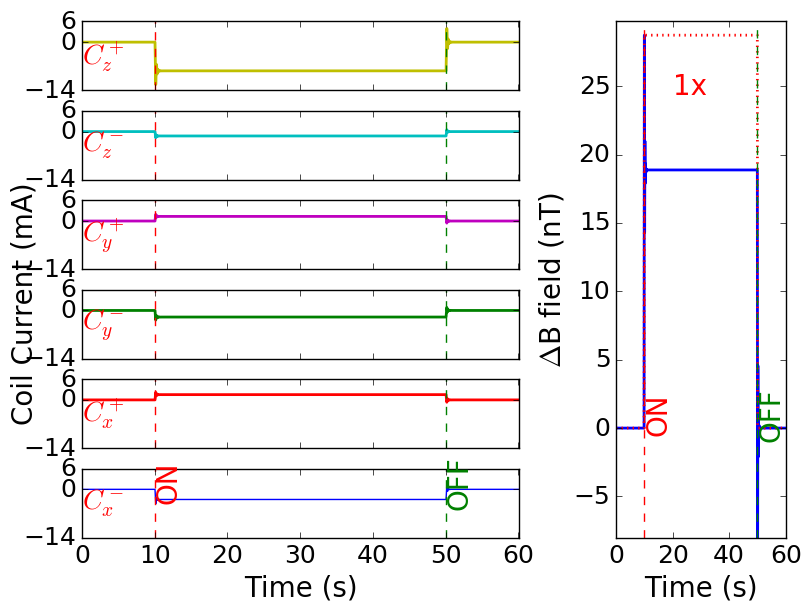
\includegraphics[width=\linewidth, height= 6.5 cm]{Images/p50}
% %         \caption{at $k_c^p$=0.50}
% %         \label{fig:p50}
% %     \end{subfigure}\\[1ex]
% %     \begin{subfigure}{.5\linewidth}
% %         \centering
% %         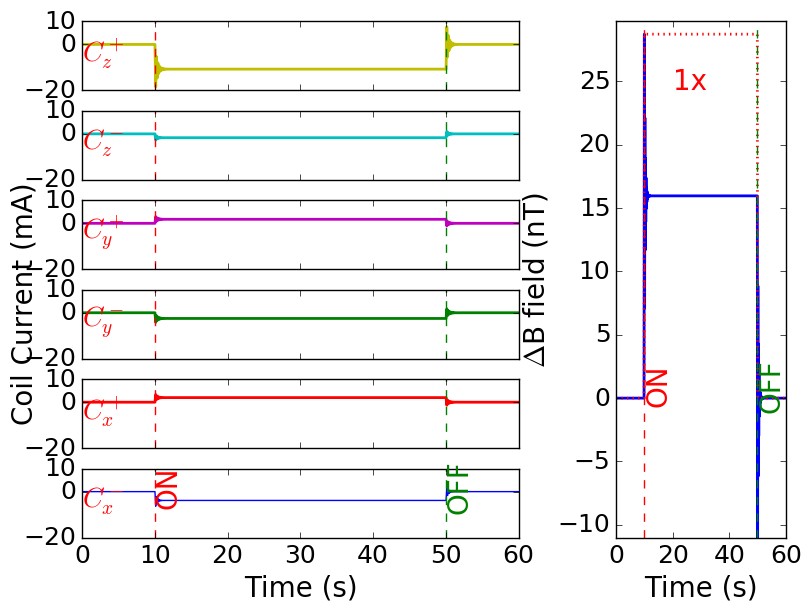
\includegraphics[width=\linewidth, height= 6.5 cm]{Images/p75}
% %         \caption{at $k_c^p$=0.75}
% %         \label{fig:p75}
% %     \end{subfigure}%
% %         \begin{subfigure}{.5\linewidth}
% %         \centering
% %         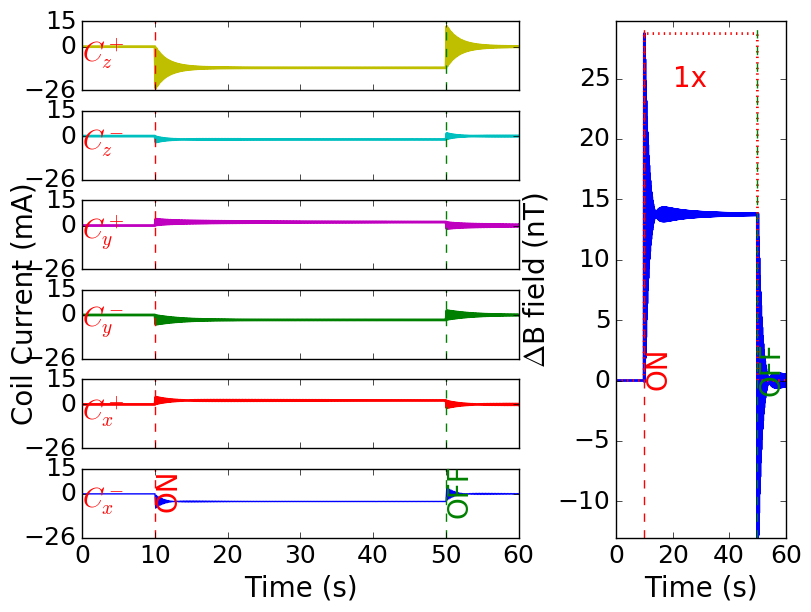
\includegraphics[width=\linewidth, height= 6.5 cm]{Images/p100}
% %         \caption{at $k_c^p$=1.0}
% %         \label{fig:p100}
% %     \end{subfigure}

% %     \caption{Currents (left vertical axis) in all six coil sides ($C_x^\pm$, $C_y^\pm$ and $C_z^\pm$) with drift $\Delta$B (right vertical axis) at sensor position '1x' for different values of $k_c^p$ with $k_c^i$ in Eq.~(\ref{eq:I}) being zero. Blue color curve denotes the actual drift in signal at position '1x' found by Eq.~(\ref{eq:del_B}) while the red curve denotes the drift that would have been without the compensation. The 'ON' and 'OFF' vertical dashed lines indicate the time of the perturbation coil being turned 'ON' and 'OFF' respectively. For position of coils and sensors see Fig.~\ref{fig:coil}. }
% %     \label{fig:p_pi}
% % \end{figure}
% \begin{figure}[!htb]
%     \begin{subfigure}{.5\linewidth}
%         \centering
%         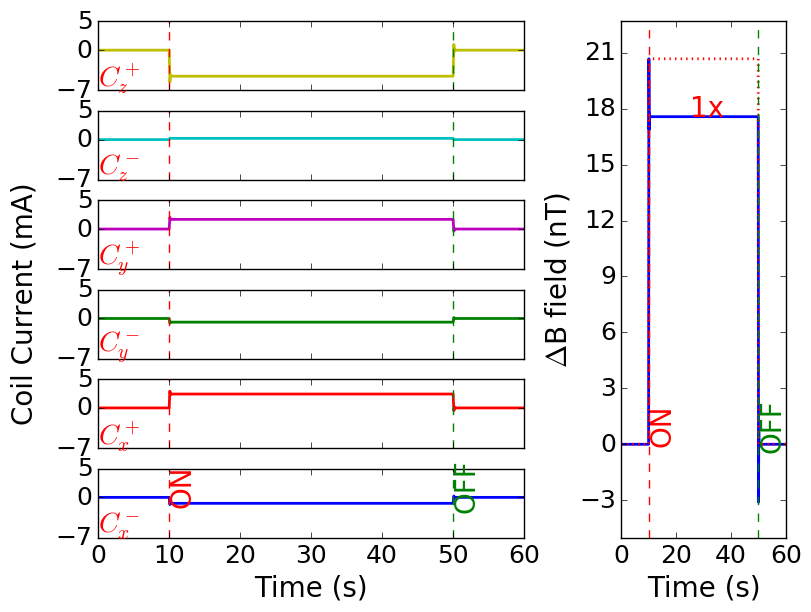
\includegraphics[width=\linewidth, height= 6.5 cm]{Images/p25_33}
%         \caption{at $k_c^p$=0.25}
%         \label{fig:p25}
%     \end{subfigure}%
%     \begin{subfigure}{.5\linewidth}
%         \centering
%         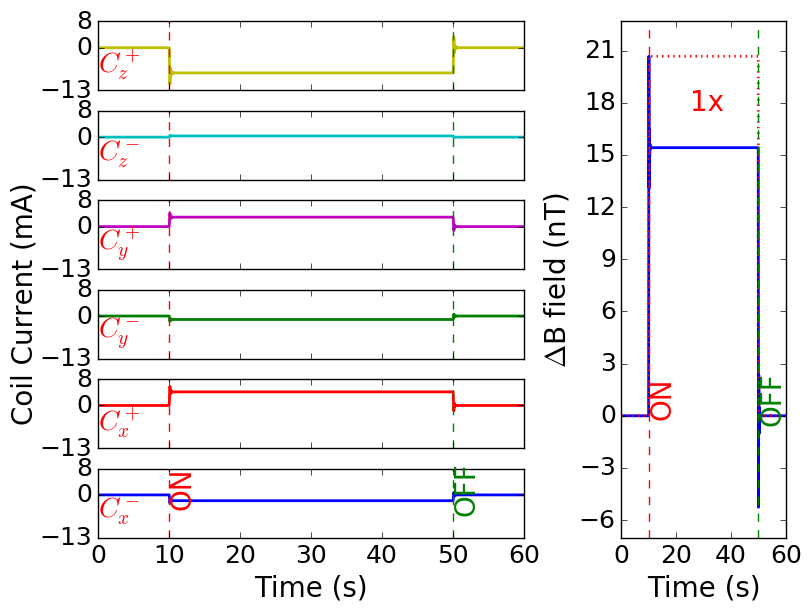
\includegraphics[width=\linewidth, height= 6.5 cm]{Images/p50_33}
%         \caption{at $k_c^p$=0.50}
%         \label{fig:p50}
%     \end{subfigure}\\[1ex]
%     \begin{subfigure}{.5\linewidth}
%         \centering
%         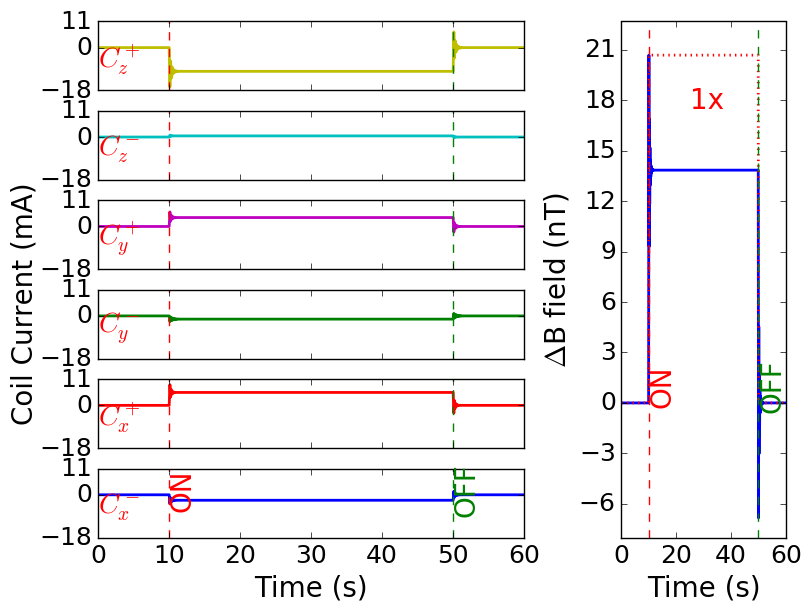
\includegraphics[width=\linewidth, height= 6.5 cm]{Images/p75_33}
%         \caption{at $k_c^p$=0.75}
%         \label{fig:p75}
%     \end{subfigure}%
%         \begin{subfigure}{.5\linewidth}
%         \centering
%         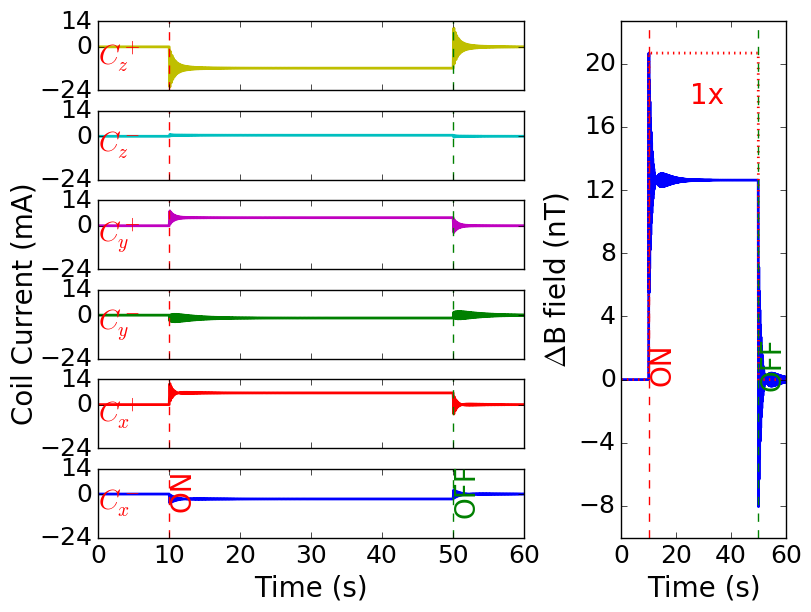
\includegraphics[width=\linewidth, height= 6.5 cm]{Images/p100_33}
%         \caption{at $k_c^p$=1.0}
%         \label{fig:p100}
%     \end{subfigure}

%     \caption{Currents (left vertical axis) in all six coil sides ($C_x^\pm$, $C_y^\pm$ and $C_z^\pm$) with drift $\Delta$B (right vertical axis) at sensor position '1x' for different values of $k_c^p$ with $k_c^i$ in Eq.~(\ref{eq:I}) being zero. Blue color curve denotes the actual drift in signal at position '1x' found by Eq.~(\ref{eq:del_B}) while the red curve denotes the drift that would have been without the compensation. The 'ON' and 'OFF' vertical dashed lines indicate the time of the perturbation coil being turned 'ON' and 'OFF' respectively. For position of coils and sensors see Fig.~\ref{fig:coil}. }
%     \label{fig:p_pi}
% \end{figure}

% The effect of changing $k_c^p$ has been shown in Fig.~\ref{fig:p_pi} where the currents (left) that are being sent to the coils ($C_x^\pm$, $C_y^\pm$ and $C_z^\pm$) for drift $\Delta$B found by Eq.~(\ref{eq:del_B}) in sensor position '1x'.  It is seen that $\Delta$B=17.5 nT, 15.5 nT and 13.5 nT for $k_c^p$ = 0.25, 0.5 and 0.75 respectively (see Fig.~\ref{fig:p_pi}\textcolor{blue}{(a)}, Fig.~\ref{fig:p_pi}\textcolor{blue}{(b)}, Fig.~\ref{fig:p_pi}\textcolor{blue}{(c)}). That is, with the increase of $k_c^p$, $\Delta$B magnetic field decreases. But, it has a limit after which with the increase of $k_c^p$, the systems becomes unstable and starts oscillating which can be seen from Fig.~\ref{fig:p_pi}\textcolor{blue}{(d)}) where the currents (left) are oscillating and the drift itself also at $\Delta$B=12.5 nT (right). So, the error is reduced maximum by (20.5-12.5)/20.5 * 100$\%\approx$37$\%$ from the initial drift of $\Delta$B=20.5 nT denoted by the red curve at position '1x'. 

% \FloatBarrier
% The above results confirm that the difference between the setpoint and the actual measurements of the magnetic field can be reduced upto a certain point. So, only having the P term is no the solution for the prototype. Next, we will discuss about the effect of only I term.

% \subsubsection{Effect of changing only I term}
% Here, the effect of changing integral reset term (I) or $k_c^i$ of Eq.~(\ref{eq:I}) will be discussed.

% The error (the difference between setpoint and actual measurement) is accumulated for the length of measurements and I term is multiplying that accumulated error  with a constant gain. For the prototype it is

% \begin{equation}
%     I_{\text{PI}}=k_c^i \sum_n \Delta I_c^n
% \end{equation}
% where, $k_c^i$ is the integral gain and $\Delta I_c^n$ is explained in Eq.~(\ref{eq:del_I}).

% Accumulated error keep tracks of the offsets that should be corrected previously. I term takes care of the offset which are not corrected by the P term and thus accelerates reducing the error level. Depending on the value $k_c^i$, how fast the feedback loop will response to the drift in the signal will be determined. A large value of $k_c^p$ will result large faster response to reducing the error level and eventually it reaches a threshold point above which the actual measurement will overshoot i.e. exceed the setpoint. 
% % The main downfall of this is that the time required for the coil current to be settle in after reducing the error level may be very slow or never ever settle in.



% % As like the effect on P, the effect of changing I has been shown in Fig.~\ref{fig:i_pi} where the change in current in all six coil sides with  $\Delta$B on a particular sensor position have been observed for $k_c^i$=0.25, 0.5, 0.75 and 1.0 . It is seen that with increase of I the level of compensation of the magnetic field is almost similar but the main difference occurs on how fast the system response in an expense of increasing current in all the coil sides (see Fig.~\ref{fig:i_pi}\textcolor{blue}{(a)}, Fig.~\ref{fig:i_pi}\textcolor{blue}{(b)}, Fig.~\ref{fig:i_pi}\textcolor{blue}{(c)} and Fig.~\ref{fig:i_pi}\textcolor{blue}{(d)}). The main problem with changing only I term is that it creates a very slow current response time. But, in terms of compensation only changing I gives very good result. The slow current response can be minimized by decreasing the value of optimized 'r' (see Section \ref{sec:r_pi} and Section \ref{sec:r_currentResponse} ).

% % \begin{figure}[!htb]
% %     \begin{subfigure}{.5\linewidth}
% %         \centering
% %         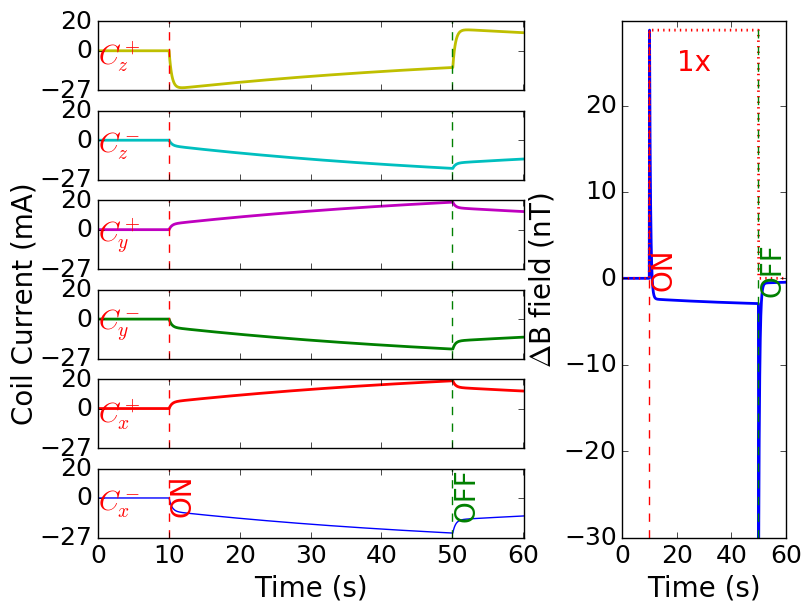
\includegraphics[width=\linewidth, height= 6.5 cm]{Images/i25}
% %         \caption{at $k_c^i$=0.25}
% %         \label{fig:i25}
% %     \end{subfigure}%
% %     \begin{subfigure}{.5\linewidth}
% %         \centering
% %         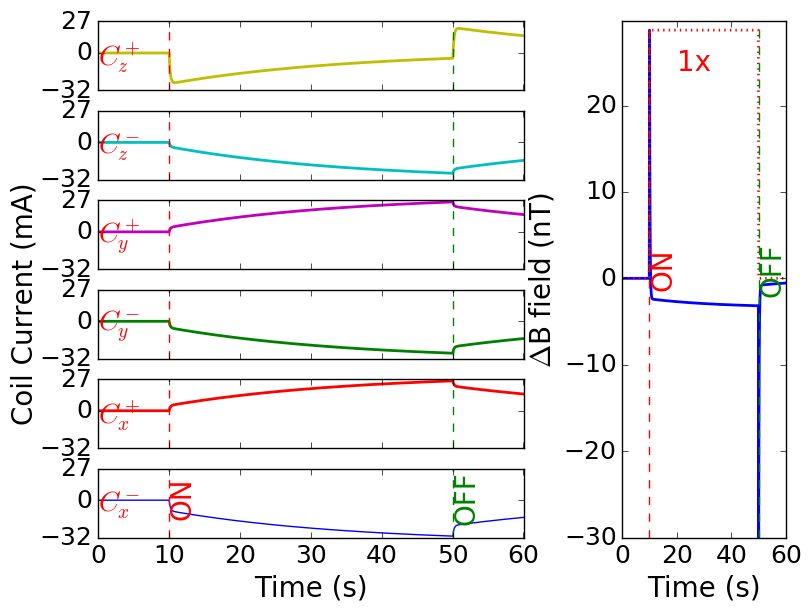
\includegraphics[width=\linewidth, height= 6.5 cm]{Images/i50}
% %         \caption{at $k_c^i$=0.5}
% %         \label{fig:i50}
% %     \end{subfigure}\\[1ex]
% %     \begin{subfigure}{.5\linewidth}
% %         \centering
% %         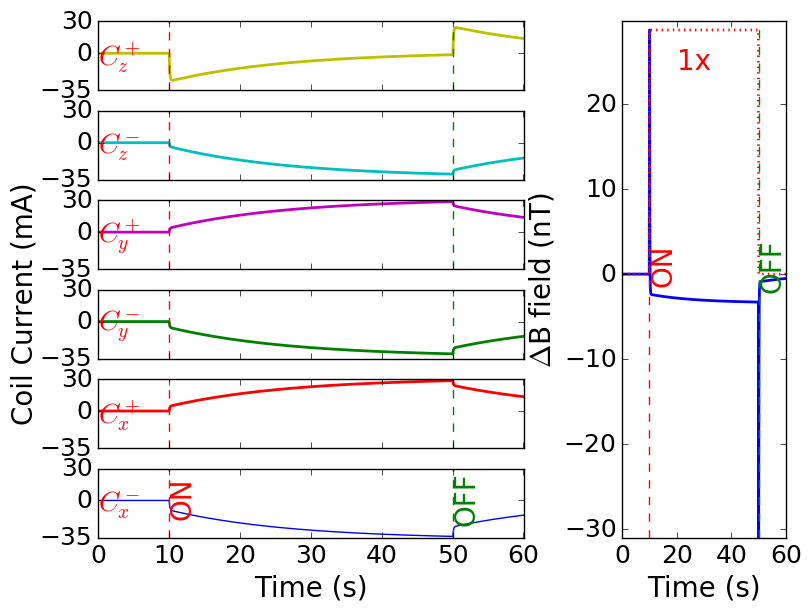
\includegraphics[width=\linewidth, height= 6.5 cm]{Images/i75}
% %         \caption{at $k_c^i$=0.75}
% %         \label{fig:i75}
% %     \end{subfigure}%
% %         \begin{subfigure}{.5\linewidth}
% %         \centering
% %         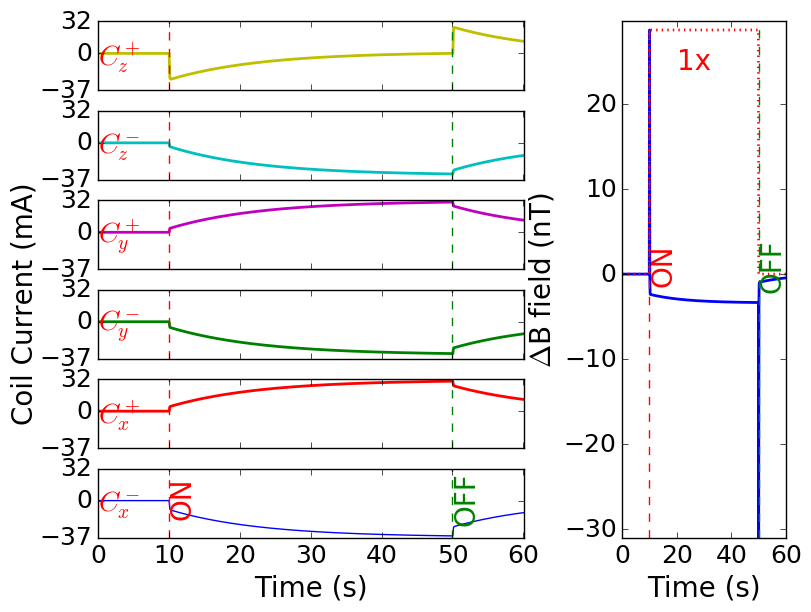
\includegraphics[width=\linewidth, height= 6.5 cm]{Images/i100}
% %         \caption{at $k_c^i$=1.0}
% %         \label{fig:i100}
% %     \end{subfigure}

% %     \caption{Currents (left vertical axis) in all six coil sides ($C_x^\pm$, $C_y^\pm$ and $C_z^\pm$) with drift $\Delta$B (right vertical axis) at sensor position '1x' for different values of $k_c^i$ with $k_c^p$ ( see Eq.~(\ref{eq:I}) ) being zero. Blue color curve denotes the actual drift in signal at position '1x' found by Eq.~(\ref{eq:del_B}) while the red curve denotes the drift that would have been without the compensation. The 'ON' and 'OFF' vertical dashed lines indicate the time of the perturbation coil being turned 'ON' and 'OFF' respectively. For position of coils and sensors see Fig.~\ref{fig:coil}.}
% %     \label{fig:i_pi}
% % \end{figure}
% \begin{figure}[!htb]
%     \begin{subfigure}{.5\linewidth}
%         \centering
%         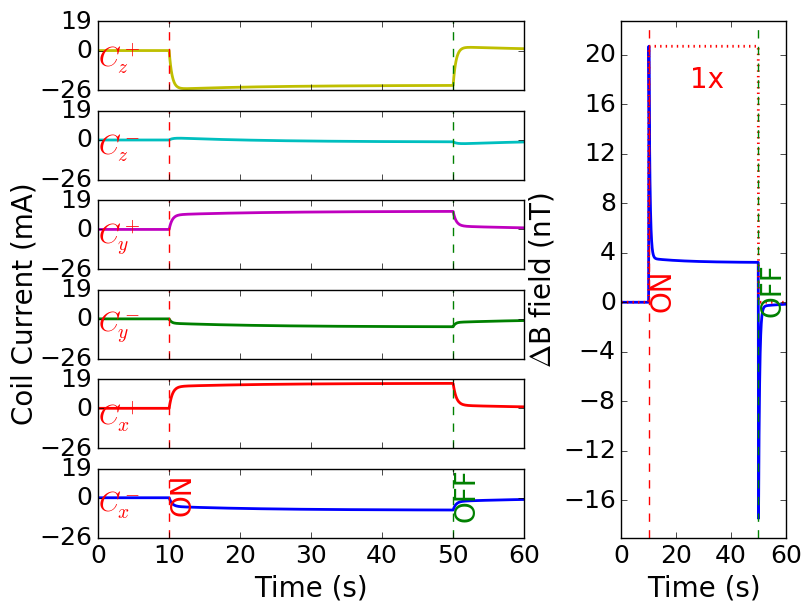
\includegraphics[width=\linewidth, height= 6.5 cm]{Images/i25_33}
%         \caption{at $k_c^i$=0.25}
%         \label{fig:i25}
%     \end{subfigure}%
%     \begin{subfigure}{.5\linewidth}
%         \centering
%         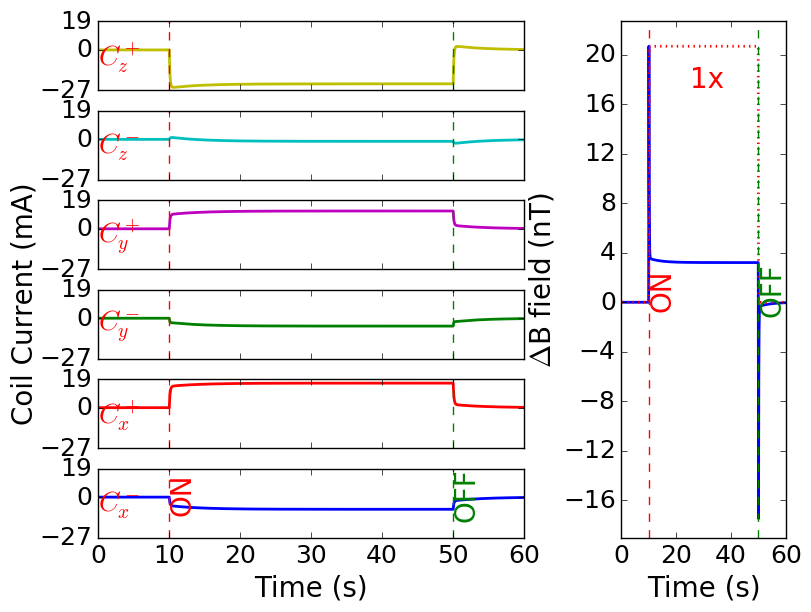
\includegraphics[width=\linewidth, height= 6.5 cm]{Images/i75_33}
%         \caption{at $k_c^i$=0.75}
%         \label{fig:i50}
%     \end{subfigure}\\[1ex]
%     \begin{subfigure}{.5\linewidth}
%         \centering
%         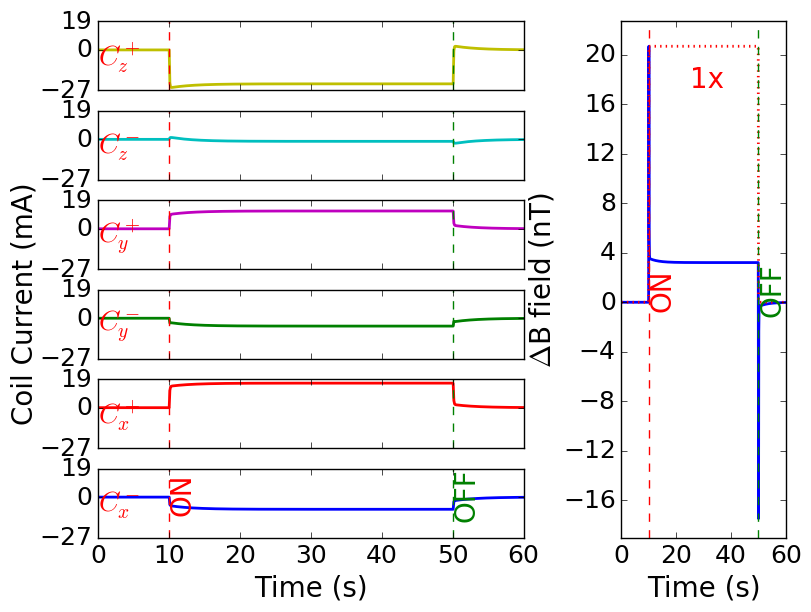
\includegraphics[width=\linewidth, height= 6.5 cm]{Images/i100_33}
%         \caption{at $k_c^i$=1.0}
%         \label{fig:i75}
%     \end{subfigure}%
%         \begin{subfigure}{.5\linewidth}
%         \centering
%         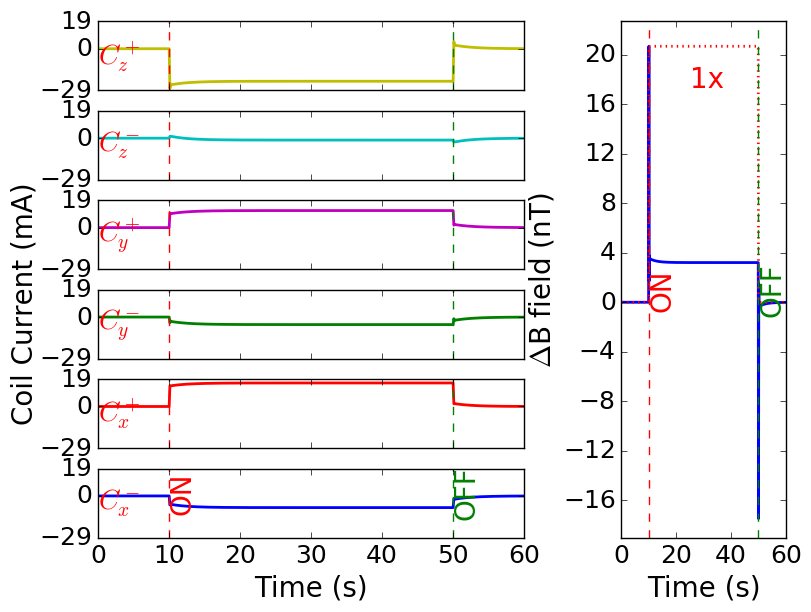
\includegraphics[width=\linewidth, height= 6.5 cm]{Images/i125_33}
%         \caption{at $k_c^i$=1.25}
%         \label{fig:i100}
%     \end{subfigure}

%     \caption{Currents (left vertical axis) in all six coil sides ($C_x^\pm$, $C_y^\pm$ and $C_z^\pm$) with drift $\Delta$B (right vertical axis) at sensor position '1x' for different values of $k_c^i$ with $k_c^p$ ( see Eq.~(\ref{eq:I}) ) being zero. Blue color curve denotes the actual drift in signal at position '1x' found by Eq.~(\ref{eq:del_B}) while the red curve denotes the drift that would have been without the compensation. The 'ON' and 'OFF' vertical dashed lines indicate the time of the perturbation coil being turned 'ON' and 'OFF' respectively. For position of coils and sensors see Fig.~\ref{fig:coil}.}
%     \label{fig:i_pi}
% \end{figure}

% \FloatBarrier
% The effect of changing $k_c^i$ has been shown in Fig.~\ref{fig:i_pi} where the currents (left) that are being sent to the coils ($C_x^\pm$, $C_y^\pm$ and $C_z^\pm$) for drift $\Delta$B found by Eq.~(\ref{eq:del_B}) in sensor position '1x'.  It is seen from Fig.~\ref{fig:i_pi}\textcolor{blue}{(a)}, Fig.~\ref{fig:i_pi}\textcolor{blue}{(b)}, Fig.~\ref{fig:i_pi}\textcolor{blue}{(c)} and Fig.~\ref{fig:i_pi}\textcolor{blue}{(d)} which are correspond to $k_c^i$ = 0.25, 0.75, 1.0 and 1.25 respectively that the error level (right) is $\sim$3.5 nT in every case, the coil currents(left) never settle in any of them. The figures are neither helpful to understand the system response time nor the overshoot effect in the $\Delta$B graph (right). So for understating those effects, the $\Delta$B graphs (right) have been zoomed in and shown in Fig.~\ref{fig:i_pi_zoom}. Now it is easily seen that the system tries to keep the error level within $\sim$ 3 nT of the setpoint which is at 0 nT as a low as 6s for $k_c^i$=0.25, then 2.2 s for $k_c^i$=0.5, 1.5s for $k_c^i$=0.75 and as fast as 0.45s for $k_c^i$=1.0 in Fig.~\ref{fig:i_pi_zoom}\textcolor{blue}{(a)}, Fig.~\ref{fig:i_pi_zoom}\textcolor{blue}{(b)}, Fig.~\ref{fig:i_pi_zoom}\textcolor{blue}{(c)} and Fig.~\ref{fig:i_pi_zoom}\textcolor{blue}{(d)} respectively. It is also seen from the Fig.~\ref{fig:i_pi_zoom}\textcolor{blue}{(d)} that there is an overshoot in the error level before it settles in. That is the error level is exceeding the target which is $\sim$3 nT of the setpoint and then it settles in.

% \begin{figure}[!htb]
%     \begin{subfigure}{.5\linewidth}
%         \centering
%         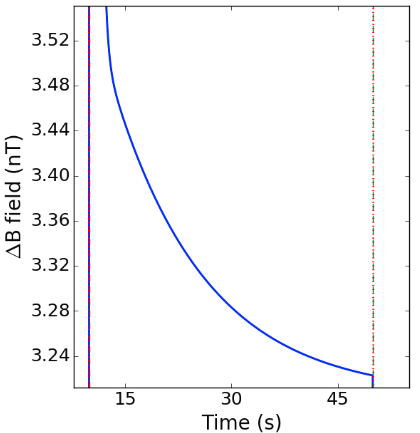
\includegraphics[width=\linewidth, height= 6.5 cm]{Images/i25_33_zoom.png}
%         \caption{at $k_c^i$=0.25}
%         \label{fig:i25zoom}
%     \end{subfigure}%
%     \begin{subfigure}{.5\linewidth}
%         \centering
%         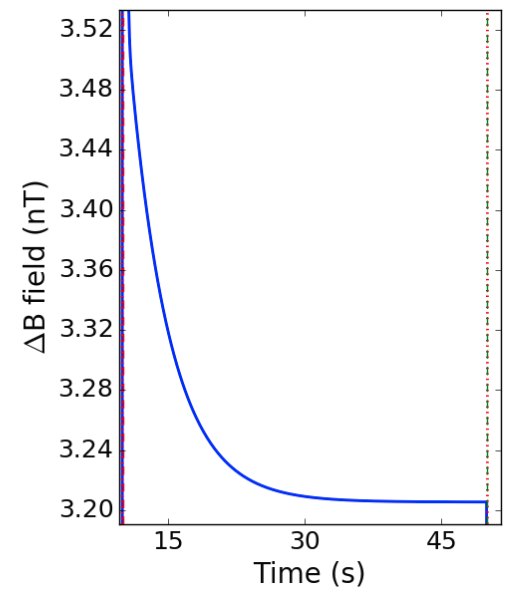
\includegraphics[width=\linewidth, height= 6.5 cm]{Images/i75_33_zoom.png}
%         \caption{at $k_c^i$=0.75}
%         \label{fig:i75zoom}
%     \end{subfigure}\\[1ex]
%     \begin{subfigure}{.5\linewidth}
%         \centering
%         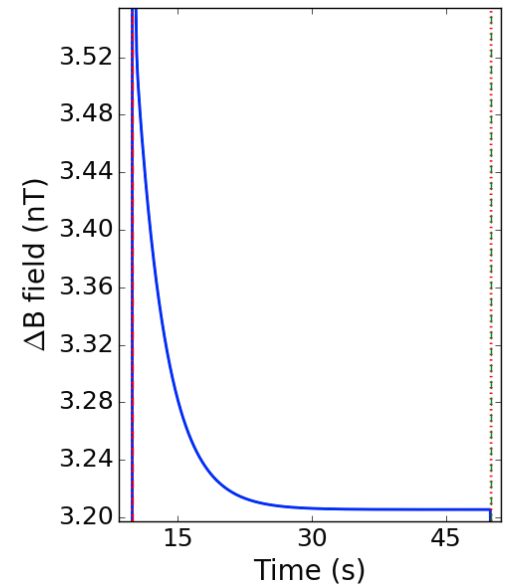
\includegraphics[width=\linewidth, height= 6.5 cm]{Images/i100_33_zoom.png}
%         \caption{at $k_c^i$=1.0}
%         \label{fig:i100zoom}
%     \end{subfigure}%
%         \begin{subfigure}{.5\linewidth}
%         \centering
%         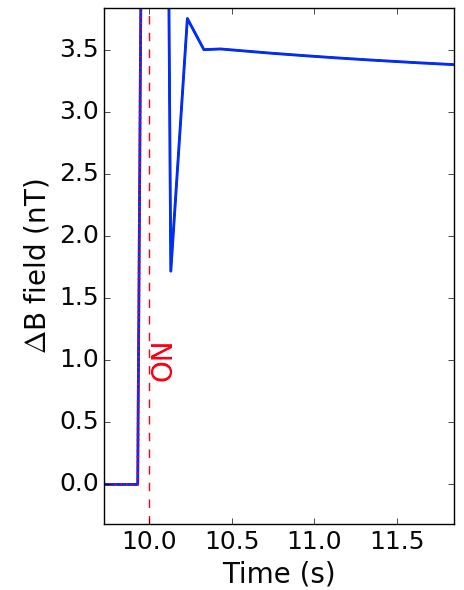
\includegraphics[width=\linewidth, height= 6.5 cm]{Images/i125_33_zoom.png}
%         \caption{at $k_c^i$=1.25}
%         \label{fig:i125zoom}
%     \end{subfigure}

%     \caption{Zoomed in version of the drift $\Delta$B shown in right side of Fig.~\ref{fig:i_pi}\textcolor{blue}{(a)}, Fig.~\ref{fig:i_pi}\textcolor{blue}{(b)}, Fig.~\ref{fig:i_pi}\textcolor{blue}{(c)} and Fig.~\ref{fig:i_pi}\textcolor{blue}{(d)} respectively at sensor position '1x' for different values of $k_c^i$ with $k_c^p$ ( see Eq.~(\ref{eq:I}) ) being zero. The red vertical dashed line indicates the time of the perturbation coil being turned 'ON'. For position of coils and sensors see Fig.~\ref{fig:coil}.\label{fig:i_pi_zoom}}
% \end{figure}

% % \fig{Images/i_pi_zoom}{width = \textwidth,height =10cm}{Zoomed in version of the drift $\Delta$B shown in right side of Fig.~\ref{fig:i_pi}\textcolor{blue}{(a)}, Fig.~\ref{fig:i_pi}\textcolor{blue}{(b)}, Fig.~\ref{fig:i_pi}\textcolor{blue}{(c)} and Fig.~\ref{fig:i_pi}\textcolor{blue}{(d)} respectively at sensor position '1x' for different values of $k_c^i$ with $k_c^p$ ( see Eq.~(\ref{eq:I}) ) being zero. The red vertical dashed line indicates the time of the perturbation coil being turned 'ON'. For position of coils and sensors see Fig.~\ref{fig:coil}.\label{fig:i_pi_zoom}}


% \FloatBarrier
% The above results confirm that to get rid of the offsets that could not be reduce by the P term, an I term is a must. But using I term shows that the currents in the coils never settles in. Next the effect of applying both of them after tuning (see Section~\ref{sec:tune}) will be discussed and may be the currents settle there!!
% % \subsection{r vs. Condition No.}\label{sec:cond}
% % Instead of going through all the steps that are discussed in section \ref{sec:inv}, the concept of condition number of a matrix can be used. The condition number of $\bm{M}$ can be determined from the diagonal matrix $\bm{\Sigma}$ as given in eq.\ref{eq:m} by -
% %  \begin{equation}
% %      cond(\bm{M})=\frac{max(\sigma_d)}{min(\sigma_d)}
% %  \end{equation}
 

% \subsubsection{Effect of changing PI term Combinely}
% Finally, the Section~\ref{sec:pi_behave} will be ended here with the discussion of the effect of changing P and I term at a time which will complete the Eq.~(\ref{eq:I}).

% Here, first the P and I term have been tuned following the discussion on Section~\ref{sec:tune} which has generated $k_c^p$=0.43 and $k_c^i$=0.52 . The results by applying $k_c^p$ and $k_c^i$ as those tuned values are shown in Fig.~\ref{fig:tuned_vs_i}\textcolor{blue}{(a)}. For simplicity instead of showing all the drift $\Delta$B for all the fluxgate sensors for the positions given in the horizonatal axis of Fig.~\ref{fig:m}, only '1x' is shown on the right of the figure. And same as earlier the currents  that are being sent to the coils ($C_x^\pm$, $C_y^\pm$ and $C_z^\pm$) shown on the left of the same figure. But, we couldn't determine the effect of having both of them at a time. So, keeping $k_c^i$ as 0.52 and excluding P term i.e. $k_c^p$=0.0 we run the same measurement again and the results are shwon in Fig.~\ref{fig:tuned_vs_i}\textcolor{blue}{(b)}. As as matter of surprise, there is hardly any difference between the results in Fig.~\ref{fig:tuned_vs_i}\textcolor{blue}{(a)} and Fig.~\ref{fig:tuned_vs_i}\textcolor{blue}{(b)}. Why is that so ? For the moment, the Fig.~\ref{fig:tuned_vs_i} suggests that may be we don't need P term at all or maybe we need different tuning methods. So, applying P and I term at a time doesn't solve our original problem of unsettle current, rather it raises another question of the necessity of the P term or importance of the tuning method describe in Section~\ref{sec:tune}. Due to lack of time, we did not further go into other tuning methods. Rather we have tried to correct our original problem of unsettle current and also discover the differences in the work between Ref.~\cite{bea} and Ref.~\cite{rawlik}.
% \doublefig{Images/p43i52_33}{width =\textwidth,height =8cm}{at $k_c^p$=0.43 and $k_c^i$=0.52. \label{fig:pi_tuned}}{Images/i52_33}{width = \textwidth,height =8cm}{at $k_c^p$=0.0 and $k_c^i$=0.52..\label{fig:i52}}{{Currents (left vertical axis) in all six coil sides ($C_x^\pm$, $C_y^\pm$ and $C_z^\pm$) with drift $\Delta$B (right vertical axis) at sensor position '1x' for combine different values of $k_c^i$ and $k_c^p$ ( see Eq.~(\ref{eq:I}) ). Blue color curve denotes the actual drift in signal at position '1x' found by Eq.~(\ref{eq:del_B}), while the red curve denotes the drift that would have been without the compensation. The 'ON' and 'OFF' vertical dashed lines indicate the time of the perturbation coil being turned 'ON' and 'OFF' respectively. For position of coils and fluxgate sensor see Fig.~\ref{fig:coil}.} \label{fig:tuned_vs_i}}

% \FloatBarrier
% The above results rather clearing our original acquisition of unsttle coil currents, give us more confusion on the effectiveness of the P term and also the tuning method. Instead of loooking more deep into tuning method, we moved our focused into regularization parameter to settle coil currents that will be presented in upcoming Section.


% \section{New Studies on Regularization Parameter}\label{sec:new_study_r}
% In Section~\ref{sec:inv} we have introduced the regularization parameter 'r' and then discussed a simulation model in Section~\ref{sec:mont} which later has been justified by comparing with experimental setup in Section~\ref{fig:mont_comp}. We have also talked about the tuning method in Section~\ref{sec:tune} and later in Section~\ref{sec:pi_behave} we have shown the the effect of the P and I term and a lot of questions arises there. Here, we will propose a new method to find 'r' based on condition number of matrix and finally we will will wrap up the Section with further tuning of optimized 'r' which will try to solve the current unsettle problems discussed in the earlier Section and 

% So, first new method to find 'r' will be discussed.

% \subsection{Regularization by Matrix Condition Number Method  }\label{sec:cond}
% Matrix Condition number ( see Eq.~(\ref{eq:cond} ) and regularization parameter 'r' ( see Eq.~(\ref{eq:minvR} ) have been introduced in Section.~\ref{sec:m} while discussing the inversion of the matrix $\bm{M}$ . Moreover, in Section~\ref{sec:mont}, a method of regularization by random fluctuation has been discussed. Here, we will propose another method of regularization using the concept of matrix condition number.
 
%  Recall from Section~\ref{sec:inv}, regularization is needed in the first place while inverse of the matrix $\bm{M}$ because $\bm{M}$ itself is ill-conditioned matrix. That means the $\bm{M}$ has a large condition number which while inverse would produce large currents in some ill-positioned places that will make the system unstable. So, it is required to have a well-conditioned  $\bm{M^{-1}}$ which implies that the condition number of $\bm{M^{-1}}$ should be small and that's what regularization has been doing. So, we introduce Eq.~\ref{eq:minvR} with various values of 'r' and each time the condition number of $\bm{M^{-1}}$ is stored. Then the optimized 'r'  has been determined by selecting the 'r' for which the condition number of $\bm{M^{-1}}$ is the minimum.
 
%  The condition number of $\bm{M^{-1}}$ for different values of 'r' has been shown in Fig.~\ref{fig:cond}. It is seen that for 'r'=0, the condition number of $\bm{M^{-1}}$=$\sim$40 that is same as the condition number of $\bm{M}$ itself. So, without regularization that is the condition number of pseudo-inverse of $\bm{M}$ would also give =$\sim$40. In regularization method, several 'r' is tried ( see Eq.~(\ref{eq:minvR}) ) and each time the condition number has been stored which are shown in the vertical axis. The red diamond symbol indicates that for 'r'=2.94, the condition number of $\bm{M^{-1}}$ is minimum and that is 3.1. That by using 'r'=2.94 in Eq.~(\ref{eq:minvR}), the condition number decrease from 40 to 3.1 which is 40/3.1$\approx$13 times of decrements. The Fig.\ref{fig:I-fluc} shows that the 'r'=2.87 compared to 'r'=2.94 that we found here. So, both method shows comparable result. This method will always produce fixed optimized 'r' for a particular  $\bm{M}$ but the method by random fluctuation (see Section~\ref{sec:mont}) will produce different optimize 'r' for different run as it because depends on the random field.

 
% \fig{Images/6c_Mcond}{width = \textwidth,height =10cm}{Condition Number of $\bm{M^{-1}}$ (vertical axis) for different values of 'r. The matrix is same as described by the Fig.~\ref{fig:m}.  \label{fig:cond}}

% \FloatBarrier

% In the above, different method to find optimize 'r' has been discussed which is a good alternative to the one explained in Section~\ref{sec:mont} and the results are similar. But it doesn't also solve the current unsettle problem discussed in Section~\ref{sec:pi_behave}. So, in the next tried again the several values of 'r' to see its effect on current unsettle problem. 


% % \subsubsection{Optimized r  Revisited Based on Current Response Time}\label{sec:r_currentResponse}
% % It was found that there is very slow coil current rise time while applying perturbation. To get rid of that problem, first and foremost, the fastest sampling frequency (see section [\ref{sec:filter}, \ref{sec:freq}]) is needed. Then, the next step of the problem can be solved via two ways with individual having own limitations. First way is tuning the value of P and I term of PI loop as explained in Eq.~(\ref{eq:I} and section \ref{sec:tune}. But with increasing the value of P, the current start oscillating after certain values as shown by the top and middle current graph on Fig.~\ref{fig:crnt} which is a problem. 

% % \fig{Images/crnt}{width = \textwidth}{Coil current in one of the coil side for optimized r=2.8 with P=0 and I=1.0 (top) and with P=0 and I=1.5 (middle) and for best r considering noise with P=0 and I=1.0 (bottom). \label{fig:crnt}}



% % The alternative way is to change the value of optimized r (see section [\ref{sec:mont}, \ref{sec:cond}]) which in turns increase noise in the prototype. But with inclusion of some current fluctuations, it was found that the coil current response time was increased heavily  as shown by the bottom current graph in Fig.~\ref{fig:crnt}. Now, the best compromised value of r was chosen by observing the 'rise time vs r' and 'fluctuations vs r' as shown in Fig.~\ref{fig:riseT}.



% %  \doublefig{Images/riseT}{width =\textwidth, height= 8 cm}{Rise Time vs r \label{fig:rise}}{Images/fluc}{width = \textwidth, height= 8 cm}{Fluctuations\label{fig:fluc}}{{(a) shows the Rise Time vs r (b) shows the Fluctuations } \label{fig:riseT}}
% % % \fig{Images/bt}{width = \textwidth}{Magnetic Field Compensation \label{fig:bt}}
% \subsection{r Behavior on PI Tuning}\label{sec:r_pi}
% % \begin{figure}[!htb]
% %     \begin{subfigure}{.5\linewidth}
% %         \centering
% %         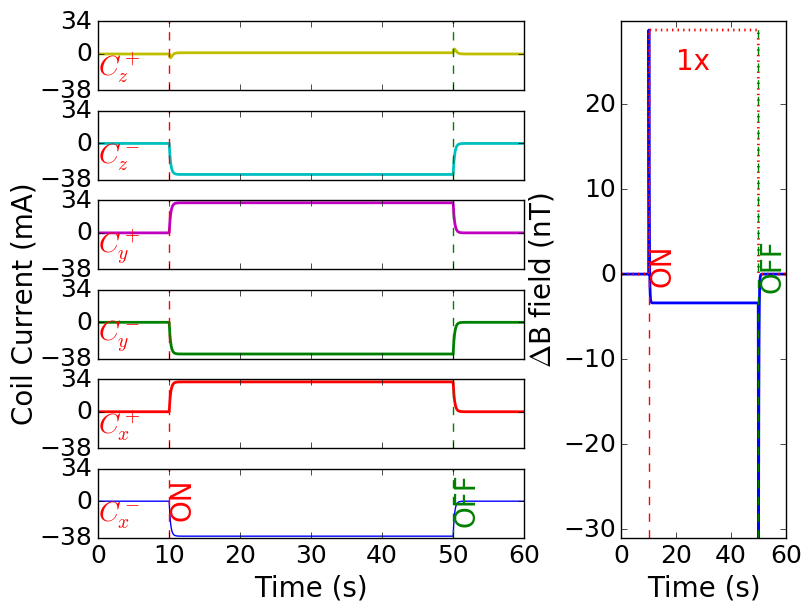
\includegraphics[width=\linewidth, height= 5 cm]{Images/r16}
% %         \caption{at r=1.6}
% %         \label{fig:r16}
% %     \end{subfigure}%
% %     \begin{subfigure}{.5\linewidth}
% %         \centering
% %         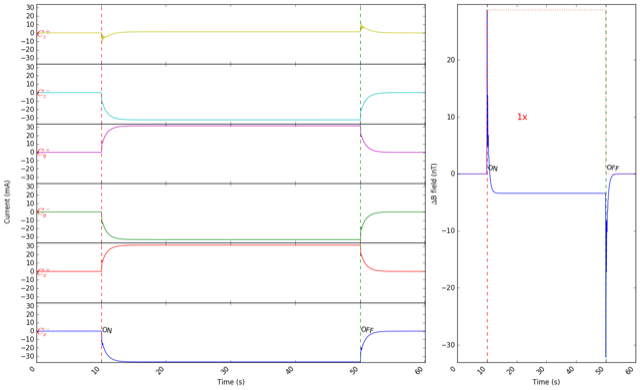
\includegraphics[width=\linewidth, height= 5 cm]{Images/r18}
% %         \caption{at r=1.8}
% %         \label{fig:r18}
% %     \end{subfigure}\\[1ex]
% %     \begin{subfigure}{.5\linewidth}
% %         \centering
% %         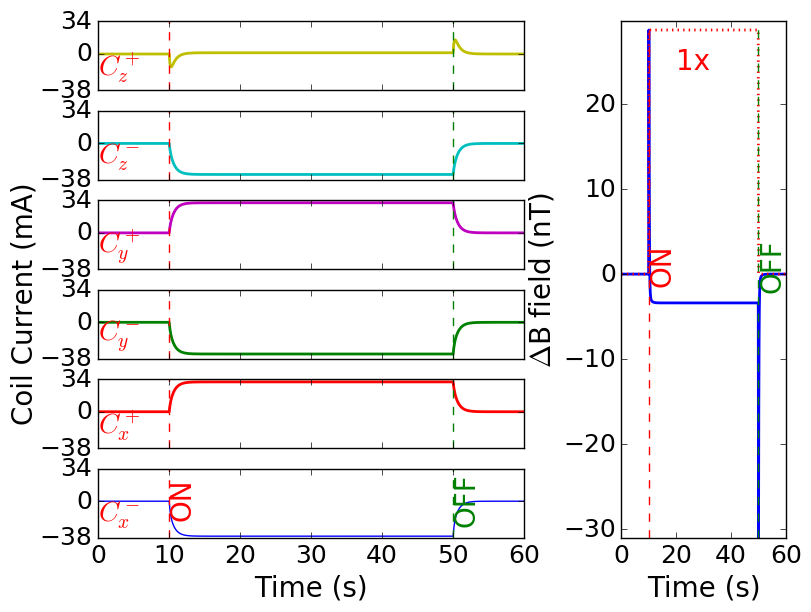
\includegraphics[width=\linewidth, height= 5 cm]{Images/r20}
% %         \caption{at r=2.0}
% %         \label{fig:fExp}
% %     \end{subfigure}%
% %         \begin{subfigure}{.5\linewidth}
% %         \centering
% %         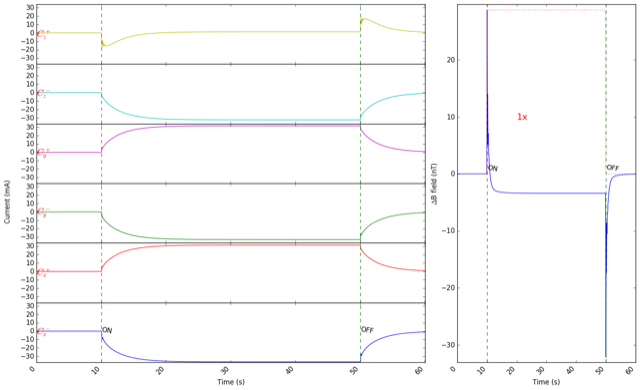
\includegraphics[width=\linewidth, height= 5 cm]{Images/r22}
% %         \caption{at r=2.2}
% %         \label{fig:r22}
% %     \end{subfigure}\\[1ex]
% %     \begin{subfigure}{.5\linewidth}
% %         \centering
% %         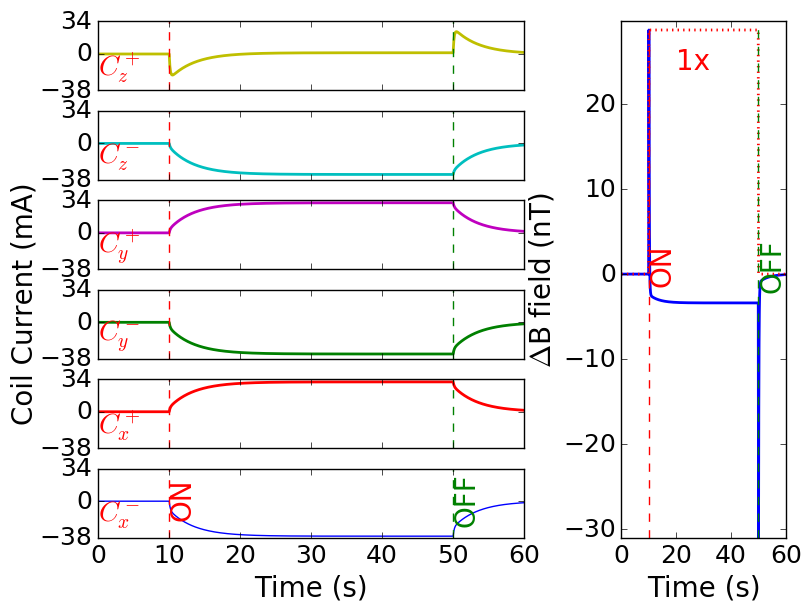
\includegraphics[width=\linewidth, height= 5 cm]{Images/r24}
% %         \caption{at r=2.4}
% %         \label{fig:r24}
% %     \end{subfigure}%
% %     \begin{subfigure}{.5\linewidth}
% %         \centering
% %         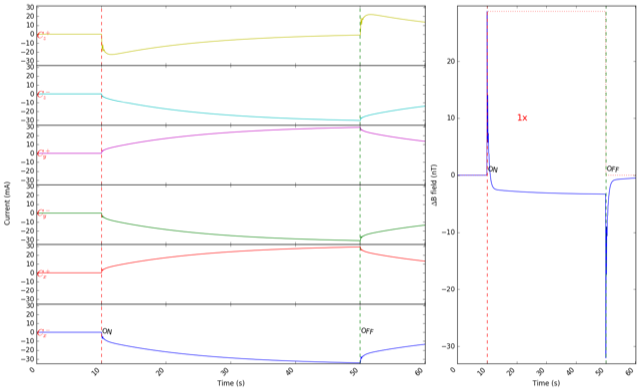
\includegraphics[width=\linewidth, height= 5 cm]{Images/r26}
% %         \caption{at r=2.6}
% %         \label{fig:r26}
% %     \end{subfigure}\\[1ex]
% %     \begin{subfigure}{.5\linewidth}
% %         \centering
% %         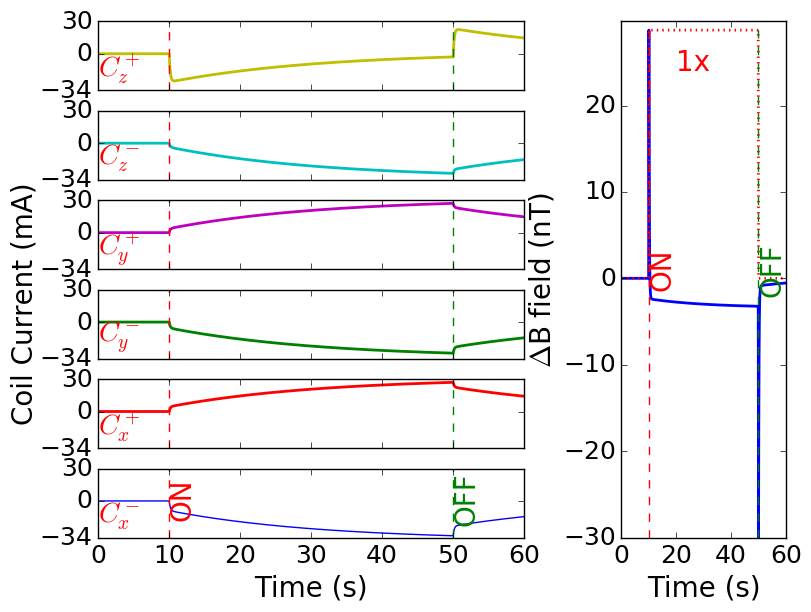
\includegraphics[width=\linewidth, height= 5 cm]{Images/r28}
% %         \caption{at r=2.8}
% %         \label{fig:r28}
% %     \end{subfigure}%
% %         \begin{subfigure}{.5\linewidth}
% %         \centering
% %         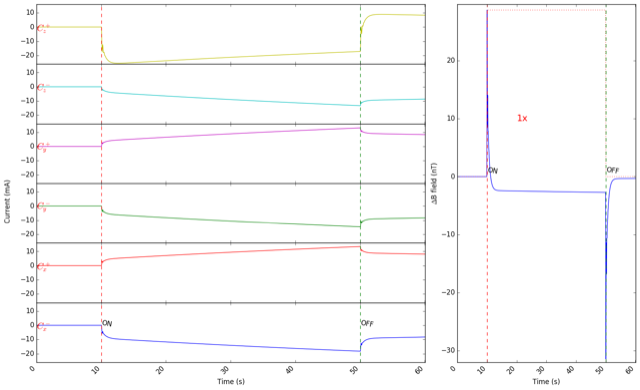
\includegraphics[width=\linewidth, height= 5 cm]{Images/r30}
% %         \caption{at r=23.0}
% %         \label{fig:r30}
% %     \end{subfigure}


% %     \caption{Change in the current in all six coil sides with obtained $\Delta$B on a particular sensor position. Here, the value of I=0.25,0.5,0.75 and 1.00 with P term being zero.}
% %     \label{fig:r_pi}
% % \end{figure}
% The discussion on Section \ref{sec:pi_behave} suggests that I term is necessary for fast system response due to any drift in the magnetic signal as it takes care of the offset problems which is unsolvable by using only P term. But, in doing so, it also creates problems in terms of the coil currents which never settle in for the duration of the perturbation. The tuning method described in Section~\ref{sec:tune} should have take care of this but we have realized that having tuned P and I has similar effect like having only I term. So, tuning method doesn't give us the solution. Rather looking for different tuning method , we have focused on the effect of 'r' on PI tuning. This Section will discuss that effect with possible outcome.

% The experimental setup is same as discussed in Section~\ref{sec:pi_behave}. But in this case we have chosen $k_c^p$=0 and $k_c^i$=0.52. Among those $k_c^i$=0.52 has been found due to PI tuning (see Section~\ref{sec:tune}) and instead of choosing  $k_c^p$=0.43 we have made this zero as from the earlier discussion we saw that it barely has any effect while we use the I term. So, these values of $k_c^p$ and $k_c^i$ will be applied on Eq.~\ref{eq:I} to find the currents to be sent to the coils ($C_x^\pm$, $C_y^\pm$ and $C_z^\pm$) for drift $\Delta$B found by Eq.~(\ref{eq:del_B}) in the sensor positions given in the horizontal axis of Fig.~\ref{fig:m}. So, keeping those fixed, we will try to change the value of 'r' which will modify the Eq.~(\ref{eq:minvR}) for each change of 'r' value.

% The effect of changing 'r' with $k_c^p$=0 and $k_c^i$=0.52 has been shown in Fig.~\ref{fig:r_pi} where the currents (left) that are being sent to the coils ($C_x^\pm$, $C_y^\pm$ and $C_z^\pm$) for drift $\Delta$B found by Eq.~(\ref{eq:del_B}) in sensor position '1x'.  It is seen from Fig.~\ref{fig:r_pi}\textcolor{blue}{(a)}, Fig.~\ref{fig:r_pi}\textcolor{blue}{(b)}, Fig.~\ref{fig:r_pi}\textcolor{blue}{(c)} and Fig.~\ref{fig:r_pi}\textcolor{blue}{(d)} which are correspond to 'r' = 2.0, 2.4, 2.8 and 3.2 respectively that the changing 'r' has significant effect on the coil current graph and barely any effect on the system response time for reducing the drift in the signal. That is at 'r'=2.0, the coil current graph has the fastest settling time where the current settles within 3 s after the perturbation has been applied. At 'r'=2.4, it takes 10s for the coil currents to settle in. But at 'r'=2.8, it seems like the coil current never settles in which is again improved at 'r'=3.2. Note that the here seroiusly ill conditioned matrix has been usedoptimized 'r' found by the simulation model is $\sim$2.9 which tells us that the coil settling of the current graph seems to have issue with the that optimized 'r. So, instead of taking the optimized 'r' that has been found by the simulation model we may have to choose the lower value of 'r'. Then question arises about what if 'r' value is chosen more than the optimized 'r'. For answering that question, we have also studied the effect for more values of 'r' with same setup which are shown in Fig.~\ref{fig:r_pi_more}. It is seen from Fig.~\ref{fig:r_pi_more}\textcolor{blue}{(a)}, Fig.~\ref{fig:r_pi_more}\textcolor{blue}{(b)}, Fig.~\ref{fig:r_pi_more}\textcolor{blue}{(c)} and Fig.~\ref{fig:r_pi_more}\textcolor{blue}{(d)} which are correspond to 'r' = 3.5, 3.6, 3.7 and 3.9 respectively that the coil current graph seems to be settle in for larger value of 'r' before it starts showing less responsive for example at 'r'=3.9 .   





% with the increase of 'r' although the error level (right) is $\sim$3 nT in every case, the coil currents(left) never settle in any of them. The figures are neither helpful to understand the system response time nor the overshoot effect in the $\Delta$B graph (right). So for understating those effects, the $\Delta$B graphs (right) have been zoomed in and shown in Fig.~\ref{fig:i_pi_zoom}. Now it is easily seen that the system tries to keep the error level within $\sim$ 3 nT of the setpoint which is at 0 nT as a low as 6s for $k_c^i$=0.25, then 2.2 s for $k_c^i$=0.5, 1.5s for $k_c^i$=0.75 and as fast as 0.45s for $k_c^i$=1.0 in Fig.~\ref{fig:i_pi_zoom}\textcolor{blue}{(a)}, Fig.~\ref{fig:i_pi_zoom}\textcolor{blue}{(b)}, Fig.~\ref{fig:i_pi_zoom}\textcolor{blue}{(c)} and Fig.~\ref{fig:i_pi_zoom}\textcolor{blue}{(d)} respectively. It is also seen from the Fig.~\ref{fig:i_pi_zoom}\textcolor{blue}{(d)} that there is an overshoot in the error level before it settles in. That is the error level is exceeding the target which is $\sim$3 nT of the setpoint and then it settles in.


% and fast response and that also causes the current in the coil sides being higher with very slow current response time. To minimize that in addition to normal tuning of PI, the effect of 'r' on PI tuning has been also studied as shown in Fig.~\ref{fig:r_pi} where the change in current in all six coil sides with  $\Delta$B on a particular sensor position have been observed for P=0.45, I=0.27 and r=1.8, 2.2, 2.6 and 3.0. It is seen that with increase of 'r' having same P and I term, the response on the current decreases (see Fig.~\ref{fig:r20}, Fig.~\ref{fig:r24}, Fig.~\ref{fig:r28} and Fig.~\ref{fig:r32}). So, the tuned system can be more tuned up by changing 'r' (more on Section \ref{sec:r_pi}). This is an unique finding as it suggests to alternative option of tuning.

% \begin{figure}[!htb]
%     \begin{subfigure}{.5\linewidth}
%         \centering
%         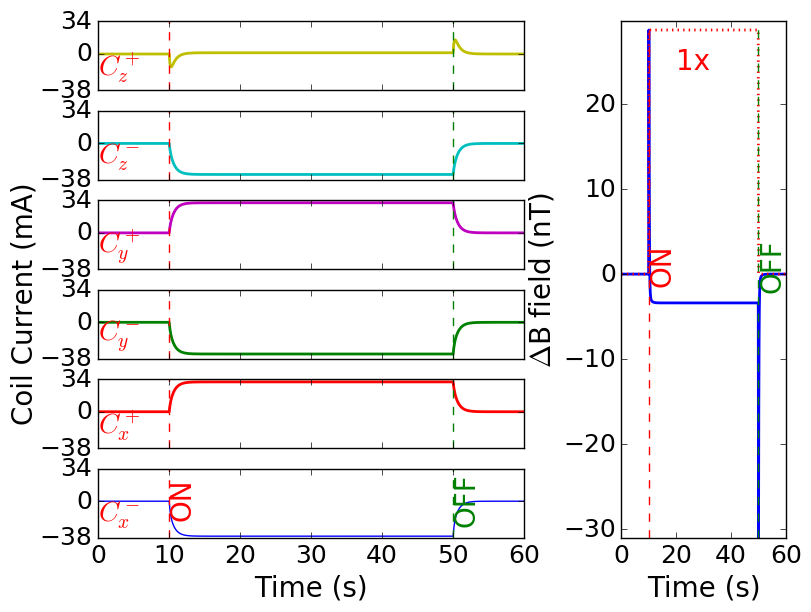
\includegraphics[width=\linewidth, height= 6.5 cm]{Images/r20}
%         \caption{at r=2.0}
%         \label{fig:r20}
%     \end{subfigure}%
%     \begin{subfigure}{.5\linewidth}
%         \centering
%         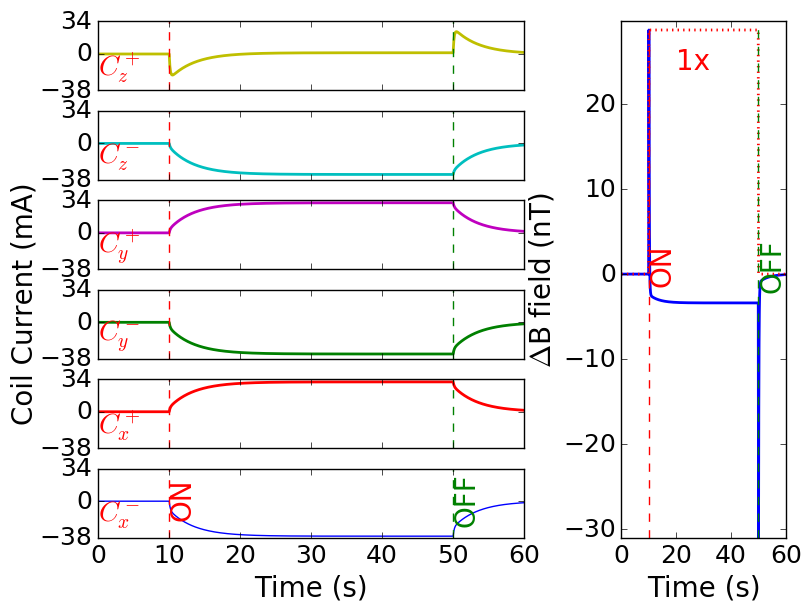
\includegraphics[width=\linewidth, height= 6.5 cm]{Images/r24}
%         \caption{at r=2.4}
%         \label{fig:r24}
%     \end{subfigure}\\[1ex]
%     \begin{subfigure}{.5\linewidth}
%         \centering
%         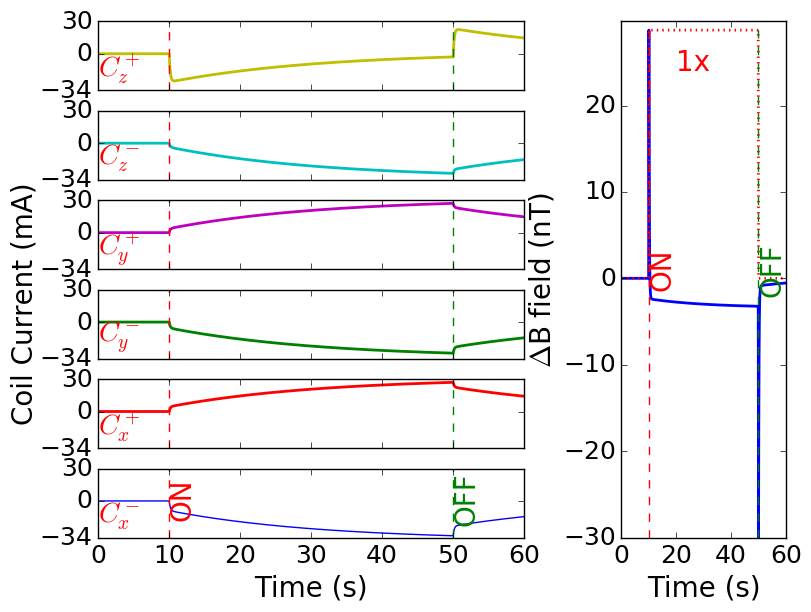
\includegraphics[width=\linewidth, height= 6.5 cm]{Images/r28}
%         \caption{at r=2.8}
%         \label{fig:r28}
%     \end{subfigure}%
%         \begin{subfigure}{.5\linewidth}
%         \centering
%         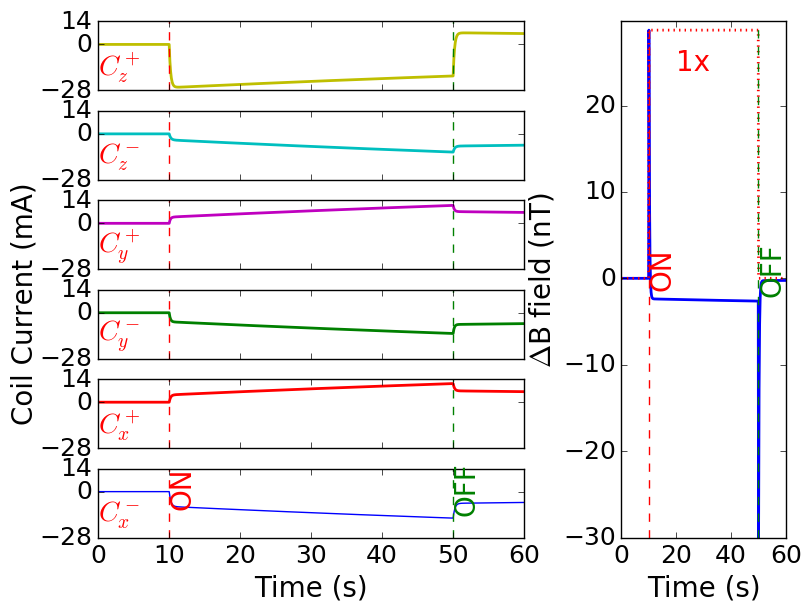
\includegraphics[width=\linewidth, height= 6.5 cm]{Images/r32}
%         \caption{at r=3.2}
%         \label{fig:r32}
%     \end{subfigure}


%     \caption{Change in the current in all six coil sides with obtained $\Delta$B on a particular sensor position with red represents uncompensated $\Delta$B. Here, the value of P=0.45, I=0.27 and r=1.8, 2.2, 2.6 and 3.0}
%     \label{fig:r_pi}
% \end{figure}
% \FloatBarrier

% \begin{figure}[!htb]
%     \begin{subfigure}{.5\linewidth}
%         \centering
%         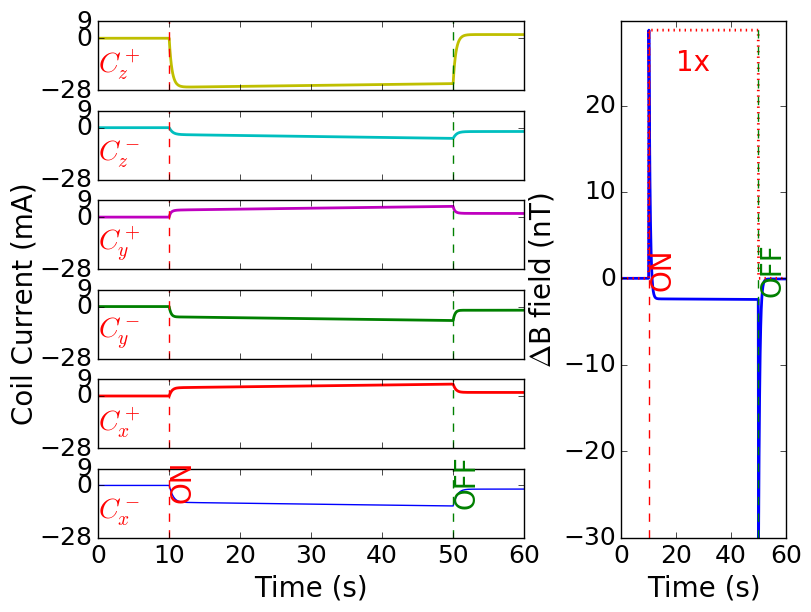
\includegraphics[width=\linewidth, height= 6.5 cm]{Images/r35}
%         \caption{at r=3.5}
%         \label{fig:r35}
%     \end{subfigure}%
%     \begin{subfigure}{.5\linewidth}
%         \centering
%         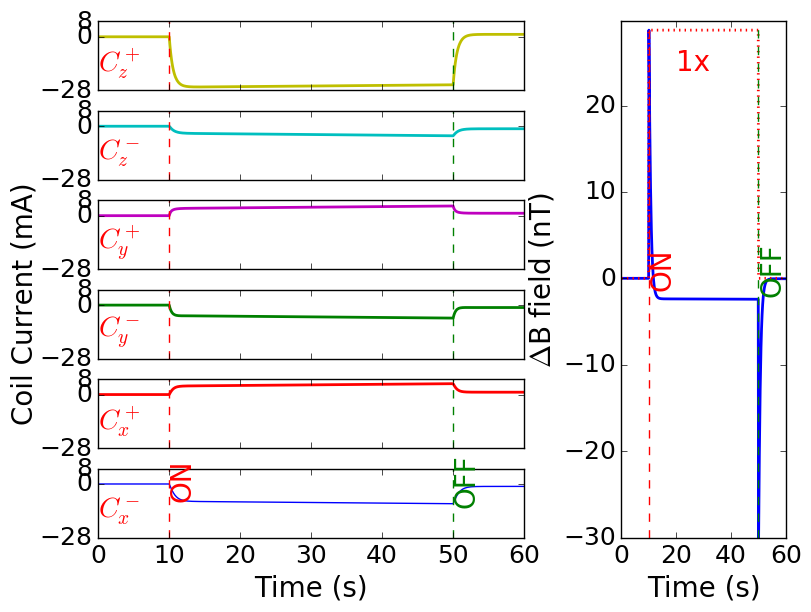
\includegraphics[width=\linewidth, height= 6.5 cm]{Images/r36}
%         \caption{at r=3.6}
%         \label{fig:r36}
%     \end{subfigure}\\[1ex]
%     \begin{subfigure}{.5\linewidth}
%         \centering
%         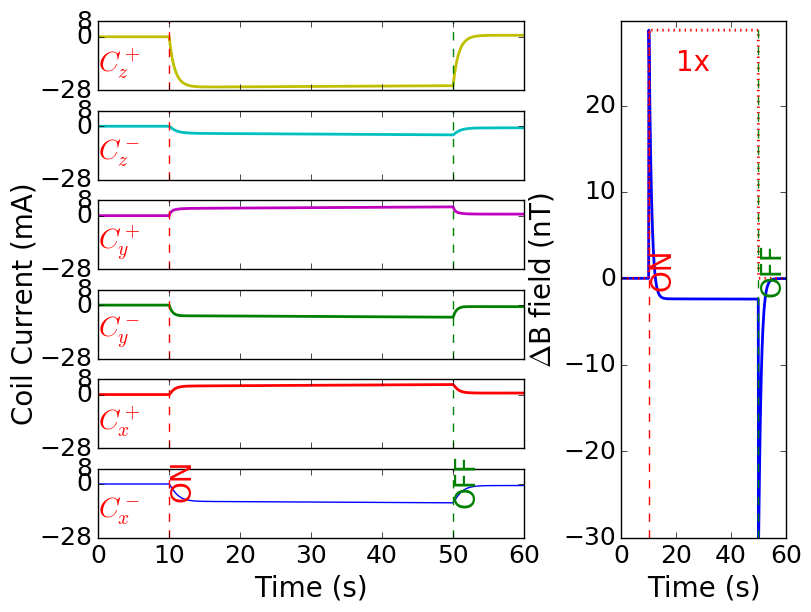
\includegraphics[width=\linewidth, height= 6.5 cm]{Images/r37}
%         \caption{at r=3.7}
%         \label{fig:r37}
%     \end{subfigure}%
%         \begin{subfigure}{.5\linewidth}
%         \centering
%         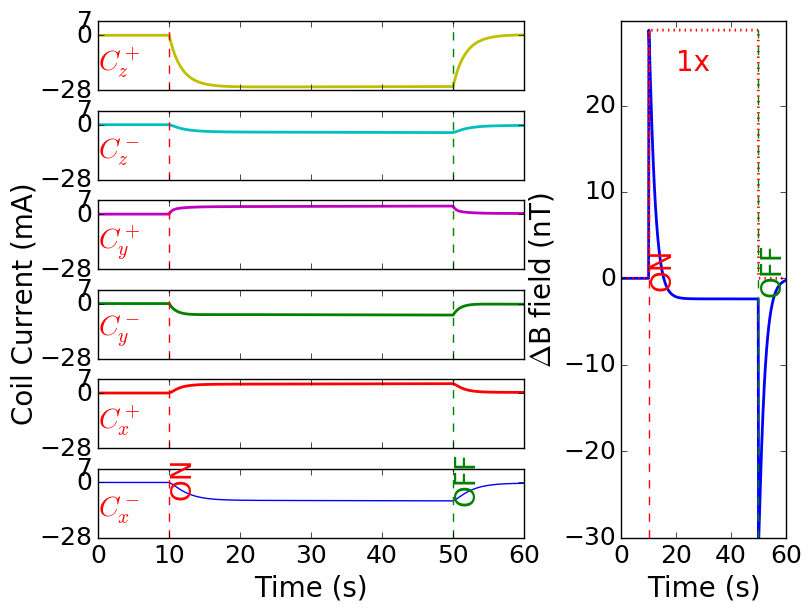
\includegraphics[width=\linewidth, height= 6.5 cm]{Images/r39}
%         \caption{at r=3.9}
%         \label{fig:r39}
%     \end{subfigure}


%     \caption{Change in the current in all six coil sides with obtained $\Delta$B on a particular sensor position with red represents uncompensated $\Delta$B. Here, the value of P=0.45, I=0.27 and r=1.8, 2.2, 2.6 and 3.0}
%     \label{fig:r_pi_more}
% \end{figure}
% \FloatBarrier
